\input{../header}
\usepackage{pgfplots}

\begin{document}
%


%\onehalfspacing
\allowdisplaybreaks
%##################################################################
\section{Chapter 1 checkpoint!}
\section{Learning target DF1, version 1}


\everymath{\displaystyle}

Suppose that you know the following values of some function $g(x)$:

\[
\begin{array}{c||r|r|r}
      x  &  1.7 &  2   &  2.3 \\\hline
    g(x) & -2.2 & -2   & -1.5
\end{array}
\]
\begin{enumerate}[leftmargin=0pt]

\item Plot these points and sketch a plausible graph of $g(x)$.

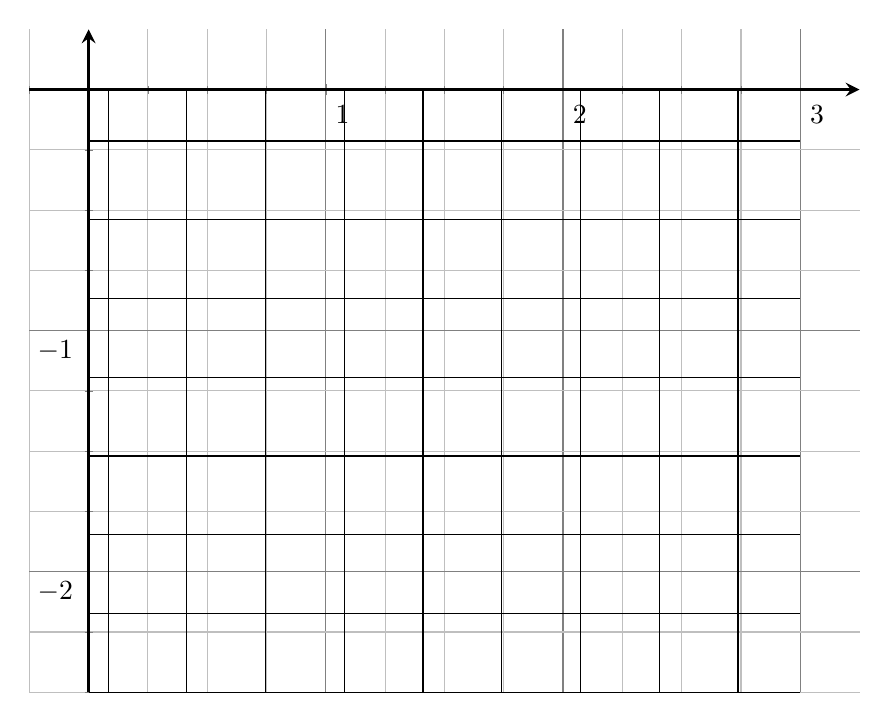
\begin{tikzpicture}
    \begin{axis}[
        width=\textwidth, height=10cm,
        xmin=-0.25, xmax=3.25, ymin=-2.5, ymax=0.25,
        xtick distance = 1, ytick distance = 1,
        minor tick num = 3,
        xticklabel style={anchor=north west},
        yticklabel style={anchor=north east},
        major grid style={thin, black!50},
        grid=both, 
        axis lines=center, axis line style = very thick]
        \draw (0,0) grid (3, -3);
    \end{axis}
\end{tikzpicture}

\item On your graph above, draw a plausible tangent line to the graph of $g(x)$ at $x=2$.

\item Use a central difference to estimate $g'(2)$. Draw the corresponding secant line on your graph above.

\vfill

\item Compute another estimate of $g'(2)$. Draw the corresponding secant line on your graph above.

\vfill

\item Which one of your approximations is the best? How do you know?

\vspace{1cm}

\end{enumerate}

%%%%%%%%%%%%%%%%%%%%%%%%%%%%%%%%%%%%%%%%%%%%%%%%%%%%%%%%%
\pagebreak
%%%%%%%%%%%%%%%%%%%%%%%%%%%%%%%%%%%%%%%%%%%%%%%%%%%%%%%%%

\section{Learning target DF2, version 1}

Suppose that $f(x) = 3x^2 - 5x + 4$.
\begin{enumerate}[leftmargin=0pt]
    \item Use the limit definition of the derivative to find $f'(x)$. \textbf{No shortcut rules!}
    
    \vfill
    \vfill

    \item Evaluate at $x=8$.

    \vfill
    \item (Bonus!) What happens to the 3? What about the $-5$? And the $4$?
\end{enumerate}

%%%%%%%%%%%%%%%%%%%%%%%%%%%%%%%%%%%%%%%%%%%%%%%%%%%%%%%%%
\pagebreak
%%%%%%%%%%%%%%%%%%%%%%%%%%%%%%%%%%%%%%%%%%%%%%%%%%%%%%%%%

\section{Learning target DFa, version 1}

A company manufactures rope, and the total cost of producing $r$ feet of rope is $C(r)$ dollars.
\begin{enumerate}[leftmargin=0pt]
    \item Suppose $C(2000) = 800$. Write a sentence explaining what this means, including units.
    \vfill
    \item What are the units of $C'(r)$?
    \vfill
    \item Suppose $C'(2000) = 0.35$. Write a sentence explaining what this means, including units.
    \vfill
    \item Do you think $C'(3000)$ is greater than, equal to, or less than $C'(2000)$? Explain why.
    \vfill
\end{enumerate}

%%%%%%%%%%%%%%%%%%%%%%%%%%%%%%%%%%%%%%%%%%%%%%%%%%%%%%%%%
\pagebreak
%%%%%%%%%%%%%%%%%%%%%%%%%%%%%%%%%%%%%%%%%%%%%%%%%%%%%%%%%

\section{Learning target DFb, version 1}

%%%%%%%%%%%%%%%%%%%%%%%%%%%%%%%%%%%%%%%%%%%%%%%%%%%%%%%%%
\pagebreak
%%%%%%%%%%%%%%%%%%%%%%%%%%%%%%%%%%%%%%%%%%%%%%%%%%%%%%%%%

\section{Learning target AD2, version 1}
Suppose that for some function \(p(x)\), you know the following information:
\begin{itemize}
    \item \(p(-2) = 5\),
    \item \(p'(-2) = 1.5\), 
    \item \(p''(x) < 0\) for \(x\)-values close to \(-2\). 
\end{itemize}

\begin{enumerate}[leftmargin=0pt]
    \item Explain and demonstrate how to find the linearization \(L(x)\) of \(p(x)\) at \(x =-2\). 
    \vfill
    \item Explain and demonstrate how to estimate the value of \(p(-2.03)\) using this linearization. 
    
    \vfill
    \item Is your estimate of \(p(-2.03)\) greater than or less than the actual value? How do you know?
    
    \vfill
    \item Sketch a possible graph of \(p(x)\) and its linearization \(L(x)\) nearby \(x =-2\) to illustrate your findings. Label important points in your sketch with their coordinates.
    
    \vfill
\end{enumerate}

\end{document}